

% Chapter 1

\chapter{Robot} % Main chapter title

\label{Chapter1} % For referencing the chapter elsewhere, use \ref{Chapter1} 

\lhead{Capítulo 1. \emph{Robot}} % This is for the header on each page - perhaps a shortened title

%----------------------------------------------------------------------------------------

\section{Desarrollo tecnológico desde Chile}

Hacer Robots en Valparaíso no es una tarea sencilla, la falta de lugares especializados para comprar dificulta contar con los componentes necesarios para construir una máquina.

Al comienzo de este proyecto se trabajó en Santiago, en conjunto con la Universidad de Chile (UChile) bajo la tutela del Doctor Juan Cristóbal Zagal en el Laboratorio de Síntesis de Máquinas Inteligentes. Por parte de la Universidad Técnica Federico Santa María (USM), se trabajó con la Doctora María José Escobar, del Departamento de Electrónica y luego se incorporó el Doctor Pablo Prieto del Departamento de Diseño de Productos. El financiamiento para realizar este prototipo ha sido por parte de las dos Instituciones, Universidad Técnica Federico Santa María y Universidad de Chile.

Durante el proceso de desarrollo se tuvieron que hacer diversas compras de materiales, pero los lugares más recurrentes al momento de hacerlas fueron Olimex y Casa Royal. La primera es una empresa dedicada a traer productos para hacer prototipos y construir máquinas, la segunda cuenta con varios insumos básicos para trabajar en desarrollo de circuitos electrónicos. Ambas empresas se encuentran en Santiago, por lo que trabajar en esta ciudad es de gran ayuda para reducir los tiempos en desarrollo.

Luego de armar un primer robot básico funcional, con materiales disponibles en Santiago de Chile, se hizo una búsqueda de componentes en tiendas especializadas que permiten comprar por internet. Existen varias (ver anexo 1) pero las más importantes para este proyecto fueron: Sparkfun y Seeedstudio.


%----------------------------------------------------------------------------------------

\section{¿Qué es un robot?}

Un robot puede ser un software solamente o tener además una extensión física que le permita interactuar con la realidad y realizar tareas de forma autónoma. Etimológicamente, el término robot se le atribuye al dramaturgo checo Karel Čapek, que en su obra R.U.R en 1921 (Rossum’s Universal Robots) utilizó la palabra “robotnik” para referirse a ayudantes artificiales. Luego fue el escritor Isaac Asimov (1920-1992) quien,  gracias a su obra, difundió la palabra robótica haciendo referencia a la ciencia encargada de estudiar a los robots. La robótica contempla el estudio de al menos 6 áreas: La mecánica, la electrónica, el control automático, la física y la matemática.

En la historia hay varios intentos por construir estos ayudantes artificiales. A principios del siglo XVIII, Jacques de Vaucanson creó un autómata capaz de tocar la flauta, así como un pato mecánico que continuamente seguía su ciclo biológico.

\begin{figure}[htbp]
	\centering
		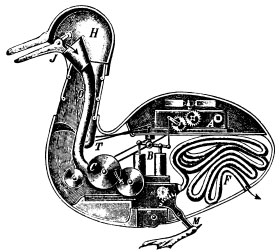
\includegraphics{./Figures/Duck_of_Vaucanson.jpg}
		\rule{35em}{0.5pt}
	\caption[Digesting Duck]{Digesting Duck, creado por Jacques de Vaucanson en 1739. Imagen extraida de Wikipedia.}
	\label{fig:Duck}
\end{figure}

En la actualidad las empresas KUKA, Honda y Sony, entre otras, construyen robots especialmente diseñados para la industria. Los robots que se utilizan en la industria, y los pocos que han llegado al hogar, son controlados por un algoritmo. Este es parte de un software que escribe una persona, donde se detalla la tarea que el robot debe realizar; tiene un modelo de los motores, partes y piezas para que así la máquina tenga información de como es, y pueda ejecutar la tarea para la cual se le programó. Si se interfiere con el entorno del robot, por ejemplo moviendo 1 [cm], fuera del rango de los sensores, el perno que debe apretar algún robot industrial que ensambla autos, este no podrá “encontrarlo”. Los robots comerciales que existen hoy en día no son capaces de adaptarse a cambios en el entorno y menos ser capaces de generar una imagen de sí mismos que les permita entender qué sucede y recuperarse de fallas.

\begin{figure}[htbp]
	\centering
		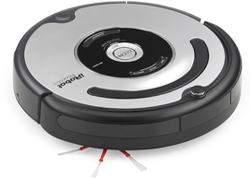
\includegraphics[width=0.4\textwidth]{./Figures/roomba.png}
		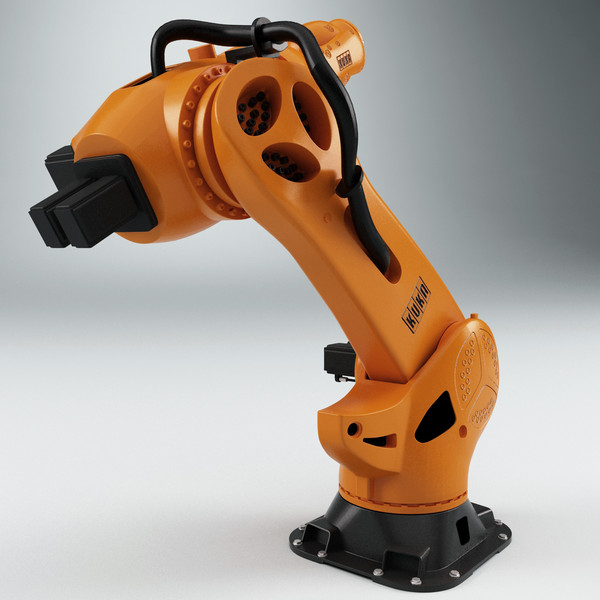
\includegraphics[width=0.4\textwidth]{./Figures/PR_KR1000_titan_01.jpg}
		\rule{35em}{0.5pt}
	\caption[Roomba y KUKA]{\textbf{Izquierda:} Robot Roomba, primer Robot domestico vendido en chile, Imagen extraida de http://www.irobotchile.cl. \textbf{Derecha:} Robot industrial KUKA KR 1000 TITAM, Imagen extraida de http://www.turbosquid.com.}
	\label{fig:Roomba y KUKA}
\end{figure}

Un algoritmo debe tener un modelo detallado de los motores y sensores que posee el robot, y es tarea del programador hacer la abstracción necesaria para poder darle sentido al movimiento del conjunto de motores. Si hablamos de un robot de 4 extremidades, el programador debe ser capaz de indicar la secuencia de activación de cada motor para así  primero hacer que el robot mueva una extremidad y luego con la suma de las 4 lograr desplazarse.

\subsection{Automodelamiento}

Juan Cristobal Zagal y Hod Lipson \cite{ZagalL09} exploraron el comportamiento de un robot capaz de entrar en un proceso de self-reflection. Ellos estudiaron a un robot al cual se le programaron dos controladores, uno primitivo (primitive controller) y uno reflexivo (reflective controller) que puede observar al primero.

\begin{figure}[htbp]
	\centering
		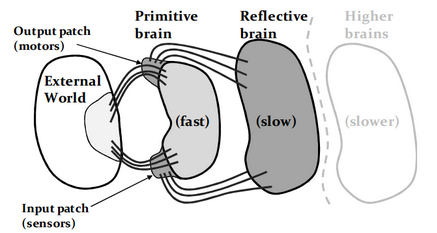
\includegraphics[width=0.7\textwidth]{./Figures/arquitectura_cerebro.png}
		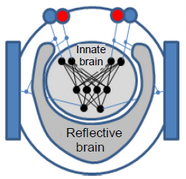
\includegraphics[width=0.4\textwidth]{./Figures/automodelado_epuck.png}
		\rule{35em}{0.5pt}
	\caption[Automodelado]{\textbf{Arriba:} Arquitectura de cerebros anidados usado en el trabajo de J.Zagal y H.Lipson, basado en modelos de M. Minsky. \textbf{Abajo:} Modelo de cerebros implementado en robot e-puck. Ambas imágenes  pertenecen a Juan Cristóbal Zagal.}
	\label{fig:Automodelado}
\end{figure}

El controlador reflexivo es capaz de determinar el control primitivo sin tener acceso directo  a sus estados internos si no que haciendo uso de ingeniería inversa al leer los input/output de éste. Acá se implementa como comportamiento que el robot (e-puck) debe alejarse de luces rojas y acercarse a azules. Se logra con una exploración mínima posible de hardware.

\begin{figure}[htbp]
	\centering
		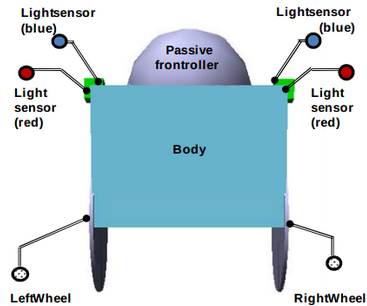
\includegraphics[width=0.4\textwidth]{./Figures/robotTest.png}
		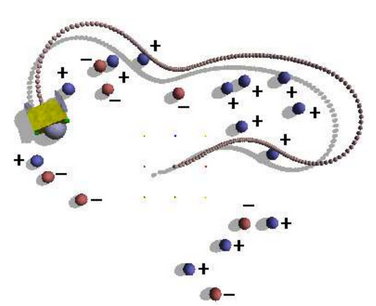
\includegraphics[width=0.5\textwidth]{./Figures/implementacion.png}
		\rule{35em}{0.5pt}
	\caption[Automodelado]{\textbf{Izquierda:} Arquitectura de cerebros anidados usado en el trabajo de J.Zagal y H.Lipson, basado en modelos de M. Minsky. \textbf{Derecha:} Modelo de cerebros implementado en robot e-puck. Ambas imágenes  pertenecen a Juan Cristóbal Zagal.}
	\label{fig:AutomodeladoTest}
\end{figure}


El diagrama del algoritmo que controla todo el proceso que se implementa como comportamiento para recuperarse de fallas puede verse en el anexo.

J. Bongard., V. Zykov y H. Lipson., logran que un robot se recupere de una falla inesperada de forma autónoma. Dicen que el robot puede recuperarse de manera autónoma haciendo uso de su (propio al robot) Self-modeling. Concretamente implementan sus algoritmos en un robot de 4 patas que utiliza una relación entre sus sensores y motores para indirectamente inferir su propia estructura.


Si se remueve una extremidad, el robot es capaz de generar una nueva forma de caminata que le permita cumplir con su misión que es avanzar.
En la figura \ref{fig:AutomodeladoLIPSON}, se describe un esquema del algoritmo. El robot realiza una acción física (A), al azar, luego se ejecuta la mejor acción que se encuentre en (C). A continuación genera varios auto-modelos que coincidan con las lecturas de los sensores obtenidas en (B). Aún no sabe cual es el modelo, por lo que en (C) genera varias acciones posibles que acotan la búsqueda de modelos.Después de varios ciclos de (A) a (C),  el modelo obtenido se utiliza en (E) para generar la secuencia de locomoción. La mejor secuencia de locomoción es probada físicamente en el robot. Se refina el modelo volviendo al paso (B) y en (D) pueden crearse nuevos comportamientos.

\begin{figure}[htbp]
	\centering
		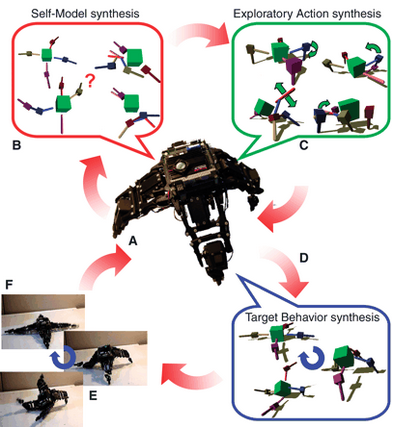
\includegraphics[width=0.5\textwidth]{./Figures/algoritmo_automodelo.png}
		\rule{35em}{0.5pt}
	\caption[AutomodeladoLIPSON]{Esquema del algoritmo que puede usar un robot para desplazarse haciendo uso de Automodelos. Imagen obtenida desde http://creativemachines.cornell.edu}
	\label{fig:AutomodeladoLIPSON}
\end{figure}

%----------------------------------------------------------------------------------------


